\subsection{2.1 Feldlinien}
    Elektrisches Feld immer tangential an Feldlinie
    \begin{tabular}{c c c}
        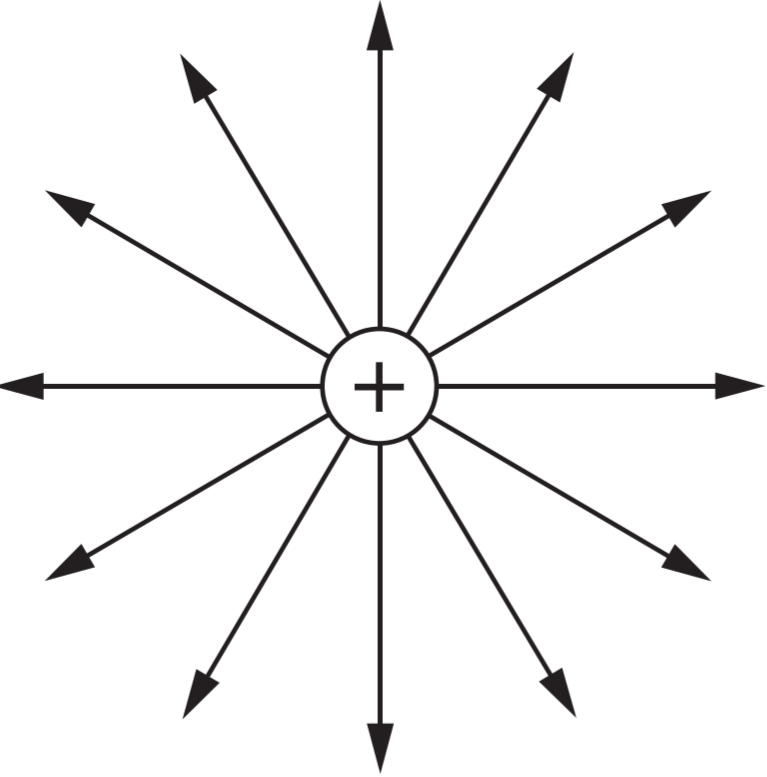
\includegraphics[height = 20mm]{src/images/punktladung.png} & 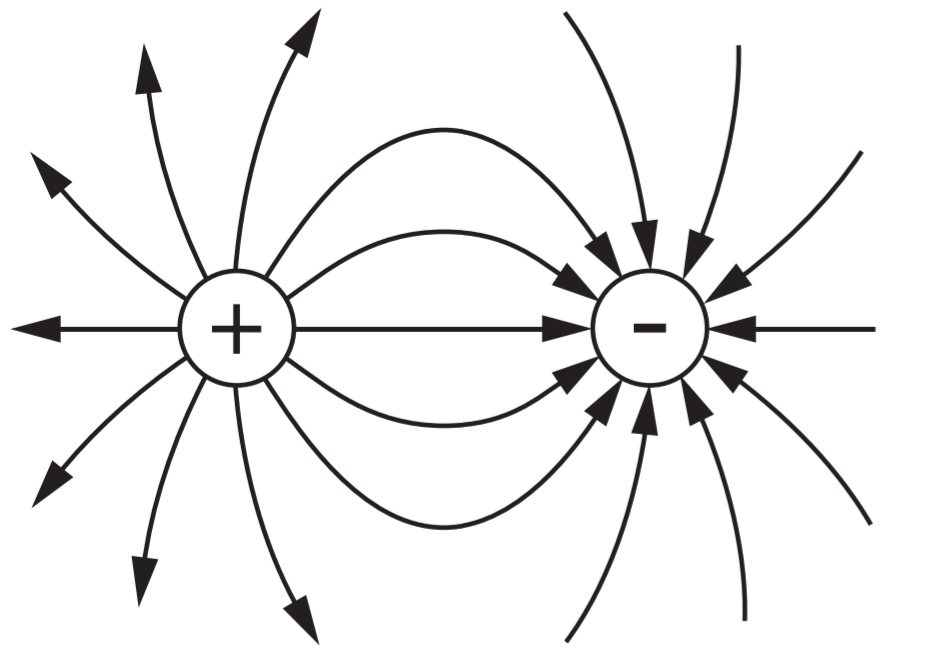
\includegraphics[height = 20mm]{src/images/zwei_punktladung.png} & 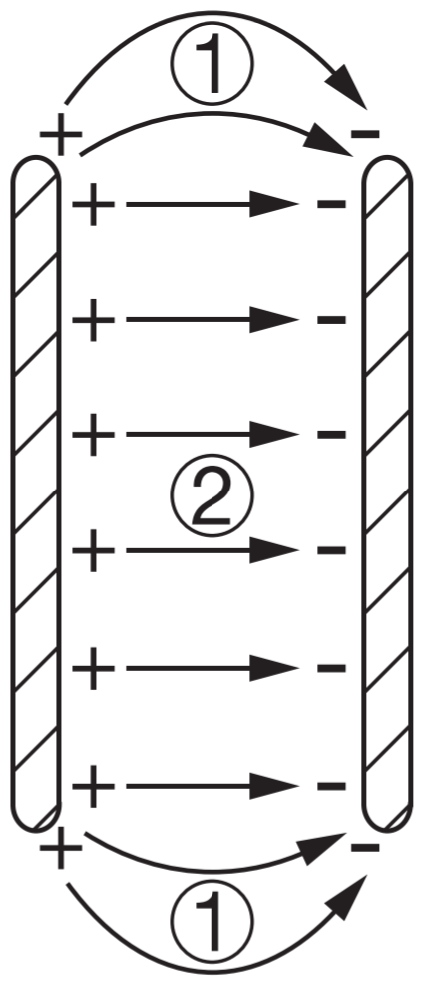
\includegraphics[height = 30mm]{src/images/kondensator.png}
    \end{tabular}

    \subsubsection*{Elektrische Feldstärke}
        \mathbox{\overrightarrow{E} = \frac{U}{l} \overrightarrow{e}} mit e Einheitsvektor in Richtung der Feldlinien

    \subsubsection*{Verschiebungsdichte}
        \mathbox{\overrightarrow{D} = \frac{Q}{A} \overrightarrow{e}}
        Im Vakuum: $\overrightarrow{D} = \varepsilon_0 \cdot \overrightarrow{E}$\\